%%%%%%%%%%%%%%%%%%%%%
% 3章
%%%%%%%%%%%%%%%%%%%%%
\chapter{ZDDを用いた区割列挙手法} \label{chapter:3}

本章では,ZDDと呼ばれるデータ構造について解説し,
川原らが提案した頂点重み格差を考慮した部分グラフ列挙アルゴリズム\cite{kawahara}
を選挙区割問題に適応する手法について述べる.

\section{ゼロサプレス型二分決定グラフ}
ゼロサプレス型二分決定グラフ(ZDD)は,組合せ集合を表す非巡回有向グラフで,
1993年に湊真一によって考案された\cite{minato}.
組合せ集合とは「$n$個のアイテムから任意個を選ぶ組合せ」を要素とする集合である.
$n$個のアイテムから任意個を選ぶ組合せは$2^n$通りあるので,
その組合せ集合は,$2^{2^n}$通り存在する.
例えば,$a,b,c$の3つの要素から組合せ集合を作る場合,
$\{ab, ac, c\}, \{a\}, \{\lambda, abc\}, \phi$などが挙げられる
($\lambda$は空の組合せ要素,$\phi$は空の集合を表す).

\begin{figure}[htbp]
  \begin{minipage}[b]{0.48\hsize}
    \centering
    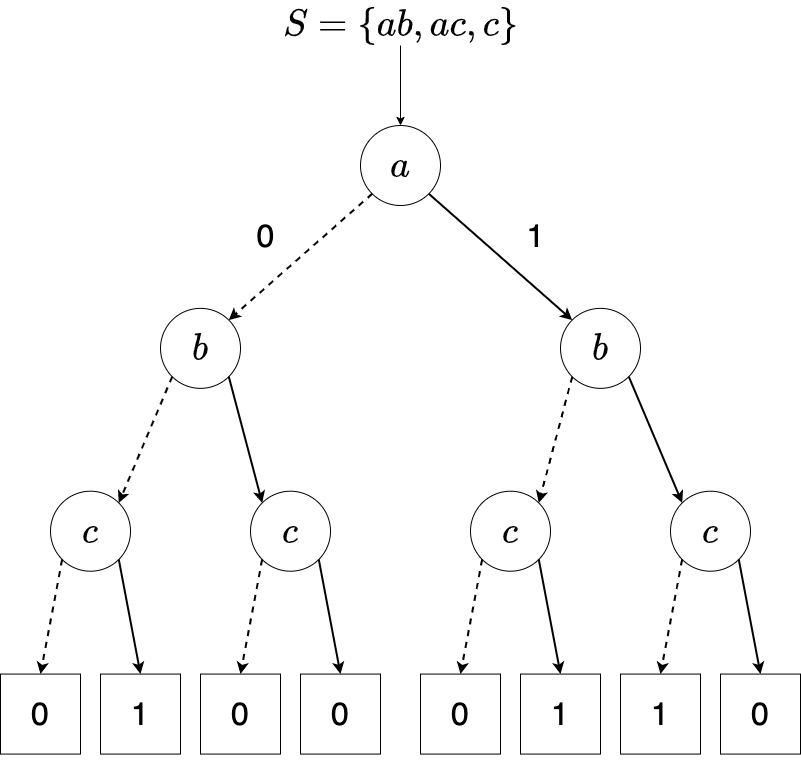
\includegraphics[scale=0.25]{img/binary_graph.png}
    \subcaption{場合分け二分木}
    \label{binary_graph}
  \end{minipage}
  \begin{minipage}[b]{0.48\hsize}
    \centering
    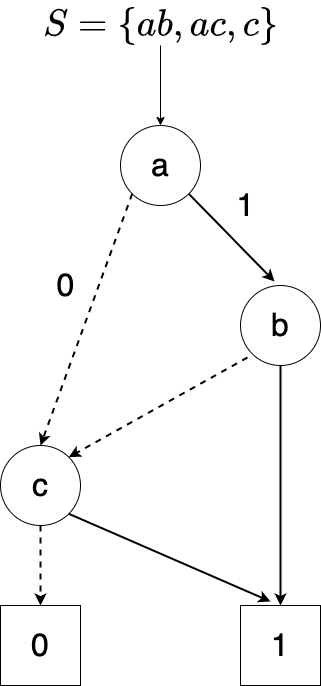
\includegraphics[scale=0.25]{img/zdd.png}
    \subcaption{ZDD}
    \label{zdd_graph}
  \end{minipage}
  \caption{組合せ集合$S=\{ab,ac,c\}$のグラフ表現}\label{combined_set}
\end{figure}

このような指数的な数の集合は,ZDDを用いることで効率的に表現することができる.
図\ref{combined_set}は,組合せ集合$S=\{ab,ac,c\}$を
場合分け二分木とZDDの両方で表した例である.
この二つのグラフは,各節点にアイテム名を表すラベルが割り当てられていて,
0と1のラベルが付与された2種類の枝が分岐している.
そして葉には0または1の値が記入されている.
以降は0のラベルをもつ枝を0-枝(破線),1のラベルをもつ枝を1-枝(実線)とし,
また,0の値が記入された葉を0-終端(0-terminal),
1の値が記入された葉を1-終端(1-terminal)と呼ぶ.
これらのグラフでは,1-枝と0-枝はその接点の要素を選ぶかどうかの場合分けを表し,
葉の値はその葉に対応する組合せが集合に属するかを示している.

場合分け二分木とZDDを比較すると,
ZDDは場合分け二分木で集合の表現に不要な頂点と枝を削除,圧縮していることがわかる.
場合分け二分木からZDDを構築するには,次の2つの規則を可能な限り適用する.

\begin{description}
  \item[冗長頂点の削除] 1-枝が0-終端を指している場合に,この節点を取り除き,
  0-枝の行き先に直結させる(図\ref{delete_zdd}).
  \item[等価節点の共有] 等価な節点(ラベルが同じで,0-枝同士,1-枝同士の行き先が同じ)
  を共有する(図\ref{share_zdd}).
\end{description}

\begin{figure}[htbp]
  \begin{minipage}[b]{0.48\hsize}
    \centering
    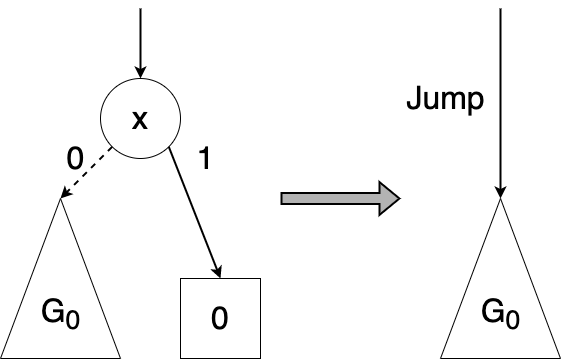
\includegraphics[scale=0.25]{img/delete_zdd.png}
    \subcaption{冗長節点の削除}
    \label{delete_zdd}
  \end{minipage}
  \begin{minipage}[b]{0.48\hsize}
    \centering
    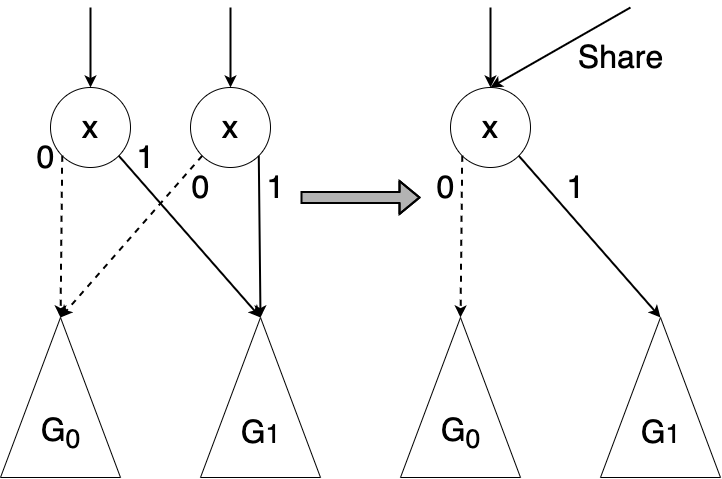
\includegraphics[scale=0.25]{img/share_zdd.png}
    \subcaption{等価節点の共有}
    \label{share_zdd}
  \end{minipage}
  \caption{ZDDの圧縮規則}\label{comp_rule}
\end{figure}

また,ZDDは組合せ集合をコンパクトに表現できるだけでなく,ZDD同士で集合演算が定義されており,
共通集合や差集合などを表すZDDを高速に得ることができる.
これを利用することで,
愚直に場合分け二分木を作るよりも高速にZDDを構築するボトムアップな構築手法\cite{minato}
が知られている.
ただし,アイテム数に対して指数的な個数の組合せを生成するような集合演算を行う場合は注意が必要であり,
集合演算の順序によっては圧縮がうまく機能せず,ZDDのサイズが指数的に増大する恐れがある.
このような場合は,計算を行う前に圧縮度を推定することは一般的に困難である.

\begin{algorithm}
  \caption{トップダウンなZDD構築アルゴリズム}
  \label{zdd_topdown}
  \begin{algorithmic}[1]
    \State 根ノード$n_{root}$を作成
    \For {$i=1,...,m$} // $m$:アイテム数
      \For {既に作成済みの$i$段目の各ノード$n$について}
      \ForAll {$x \in \{0,1\}$} // 0-枝,1-枝の処理
        \State 終端条件の判定
        \State 新しいノード$n'$を作成($i+1$段目とする)
        \State $n'$の情報を更新
        \If {$n'$と等価なノード$n''$が既に存在}
          \State $n' \gets n''$
        \EndIf
        \State $n$の$x$-枝の先を$n'$とする.
        \EndFor
      \EndFor
    \EndFor
  \end{algorithmic}
\end{algorithm}

近年の研究では,ボトムアップな構築手法ではなく,
根から順にZDDを作成するトップダウンな構築手法\cite{minato_or}\cite{sekine}
がよく用いられている.
アイテム$\{a_1,\ldots	,a_m\}$から特定の組合せ集合を表すZDDを構築するアルゴリズムについて,
疑似コードの形で\textbf{Algorithm 1}に記した.

\textbf{Algorithm 1}の2行目がZDDの格段についての処理,
3行目がその段の各ノードについての処理である.4行目が$x$-枝($x=0,1$)の先のノードを作成する.
$x=1$はアイテム$a_i$を採用する場合,$x=0$はアイテム$a_i$を採用しない場合に対応する.
5行目では,終端条件の判定を行う.その時点で組合せ集合の要素に含まれないと判定できる場合には,
$n$の$x$-枝の先を0-終端に接続する.
終端に接続する場合は,6-11行目は実行しない.
7行目では,ノードに記憶させる情報を更新する.
記憶させる情報は問題によって様々であるため,内容は後述する.
8行目でノードが共有可能であるか判定を行う.

トップダウンな構築手法では,フロンティアという
ラベル$a_i$がついた枝を処理した状態における頂点集合
$F_i=(\bigcup_{j=1,\ldots ,i}a_j)\cap (\bigcup_{j=i+1, \ldots, m} a_j)$
を用いることから,一般的に「フロンティア法」と呼ばれる.
フロンティアは,処理が途中のアイテムのみを保持するため,
\textbf{Algorithm 1}の5行目の処理では,
フロンティアに含まれるノードの情報のみ参照すればよい.
アイテムの総数に対して,フロンティアのサイズが小さければ効率よく計算を行うことができる.

なお,5-7行目の内容は,同じフロンティア法でも解く問題の種類によって細かな違いがある.
選挙区割問題の実装については後節で説明する.

\section{ZDDでの選挙区割列挙の表現}


本節では,選挙区割の列挙を表現する組合せ集合とZDDについて述べる.
選挙区割の集合は,
選挙区となる部分グラフを構築に利用できる全ての辺の組合せの集合と言い換えることができる.
例として,図\ref{kuwari}から2つの部分グラフを列挙することを考える.

\begin{figure}[htbp]
  \centering
  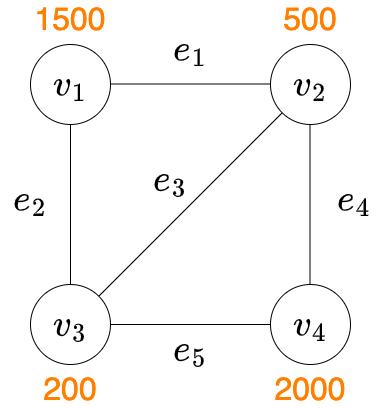
\includegraphics[scale=0.3]{img/kuwari.png}
  \caption{4頂点の重み付きグラフ}
  \label{kuwari}
\end{figure}

図\ref{kuwari}の橙色で書かれた数字は,頂点の重み,すなわち市区町村の人口である.
グラフ分割する際には,各グラフの重みをなるべく均等にしたいため,
今回は解となる頂点(市区町村)の集合を$\{\{v_1,v_2\},\{v_3,v_4\}\},
\{\{v_1,v_2,v_3\}, \{v_4\}\}$の2つとすると,
部分グラフの重みは,それぞれ$\{2000, 2200\},\{2200, 2000\}$となる.

ここで部分グラフを構成する辺に注目してみる.
頂点集合から部分グラフの構成に利用できる全ての辺の集合は,$\{e_1, e_5\}, \{e_1,e_2,e_3\}$
である.この辺集合からZDDを構築することで,選挙区割の列挙を行うことができる(図\ref{kuwari_zdd}).


\begin{figure}[ht]
  \centering
  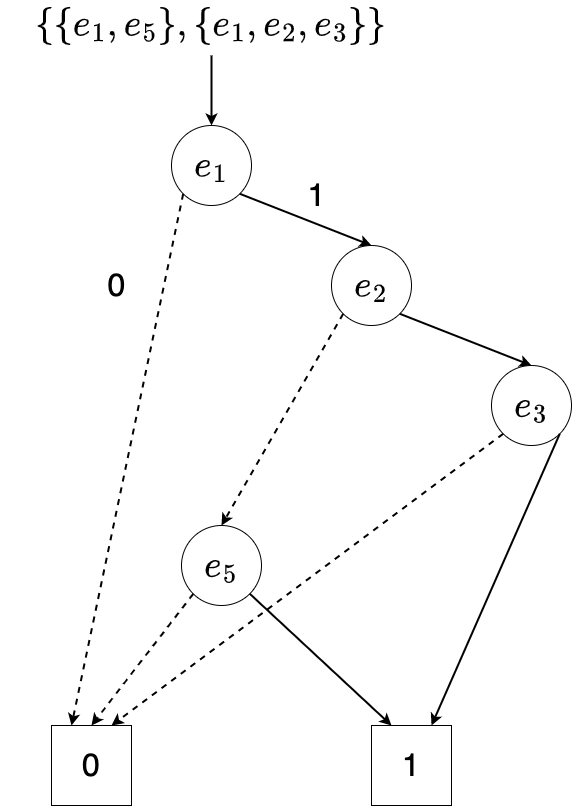
\includegraphics[scale=0.25]{img/kuwari_zdd.png}
  \caption{選挙区割の集合を表すZDD}
  \label{kuwari_zdd}
\end{figure}

図\ref{kuwari_zdd}では,節点のラベルに辺の名前が記載されている.
1-枝は節点のラベルに記されたグラフの辺を採用,
0-枝は採用しないことを表している.
そして,1-終端に向かうパスを辿ることで,求めたい部分グラフ集合を容易に見つけることができる.

\section{区割列挙アルゴリズム}
本節では,川原らが考案した重み付きグラフ分割列挙アルゴリズム\cite{kawahara}
を用いて,選挙区割を列挙するZDDの構築アルゴリズムを説明する.

アルゴリズムを説明する前準備として,用語・変数について定義する.
まず,元のグラフを$G=(V,E,w)$,辺$E$の総数を$m$,
列挙したい部分グラフ集合を$\mathcal{G}$,分割数(区割数)を$d$とする.
なお,辺集合$E$の順序付けは,ヒューリスティックアルゴリズムを用いて,
フロンティアの大きさが出来るだけ小さくなるように行う.
$N$はZDDのノードの集合を表し,$N_i$はグラフ$G$の辺$e_i (\in E)$を
ラベルにもつノード集合を指す.
$F_i$は,ラベル$e_i=\{u,v\}$をもつZDDノードを処理している地点での,
グラフの頂点集合からなるフロンティアであり,
$$ F_i=(\bigcup_{j=1,\ldots ,i}e_j)\cap (\bigcup_{j=i+1, \ldots, m} e_j) $$
から求められる.

ZDDのノード$n$には,終端を除いて以下の情報を含んでいる.

\begin{description}
  \item[$n.\mathrm{comp}$]\mbox{}\\
    フロンティア上での,部分グラフの頂点の集合を示す.\\
    例えば,$n.\mathrm{comp}=\{\{v_1,v_2,v_3\},\ldots\}$
    とあれば,頂点$v_1,v_2,v_3$が同一部分グラフの頂点であり,
    連結していることを表す.
  \item[$n.\mathrm{fps}$ ]\mbox{}\\
    接続を禁止する頂点のペアセット(forbidden pair set).\\
    例えば,部分グラフの頂点集合をそれぞれ$C_1,C_2$とすると,
    $n.\mathrm{fps}=\{\{C_1,C_2\},\ldots\}$は,
    $C_1$に含まれる頂点と$C_2$に含まれる頂点を接続させては
    いけないことを表す.
  \item[$n.\mathrm{cc}$]\mbox{}\\
    確定した部分グラフの個数の値が入る.\\
    フロンティアからある部分グラフ内の頂点が全て取り除かれたとき,
    その部分グラフは他のグラフと連結することがないため,
    $n.\mathrm{cc}$をインクリメントする.
  \item[$n.\mathrm{weight}$]\mbox{}\\
    部分グラフごとに頂点重みの和を保存する.
\end{description}

なお,根ノード$n_{root}$のもつ情報は,
$n.\mathrm{comp}$,$n.\mathrm{fps},n.\mathrm{weight}$は空集合$\emptyset$,
$n.\mathrm{cc}=1$と定義する.
次に,選挙区割のZDDを構築するフロンティア法を\textbf{Algorithm 2}に示す.

\begin{algorithm}
  \caption{ConstructZDD}
  \label{construct_zdd}
  \begin{algorithmic}[1]
    \State $N_1 \gets \{n_{root}\}$
    \State $N_i \gets \emptyset~\mathrm{for}~i=2, \ldots ,m+1$
    \For {$i=1, \ldots , m$}
      \ForAll {$n \in N_i$}
        \ForAll {$x \in \{0,1\}$}
          \State $n' \gets \mathrm{MakeNewNode}(n,i,x)$
          \If {$N' \neq \textbf{0}, \textbf{1} $}
            \If {$n'$と等価なノード$n''\in N_{i+1}$が既に存在}
              \State $n' \gets n''$
            \Else
              \State $N_{i+1} \gets N_{i+1} \cup \{n'\}$
            \EndIf
          \EndIf
          \State $n$の$x$-枝の先を$n'$とする.
        \EndFor
      \EndFor
    \EndFor
  \end{algorithmic}
\end{algorithm}

\textbf{Algorithm 2}の全体の流れは,\textbf{Algorithm 1}と大きく異ならないため,
詳細な説明は省略する.注目すべき点は,6行目の MakeNewNode という関数である.これは,
終端条件の判定と,$i+1$段目に新しいノード$n'$を作成する処理が含まれていて,新しい節点もしくは,
0-終端,1-終端のいずれかを返す.
この関数の処理を,人口制約がない場合とある場合のそれぞれで説明する.

\subsection{人口制約なしの場合}

まず,人口制約がない場合,ZDDのノードに含まれる情報は,$n.\mathrm{comp}$,$n.\mathrm{fps}$,
$n.\mathrm{cc}$の3種であり,$n.\mathrm{weight}$は含まれない.
MakeNewNode の擬似コードを\textbf{Algorithm 3}に示す.

\begin{breakablealgorithm}
  \caption{MakeNewNode}
  \label{make_new_node}
  \begin{algorithmic}[1]
    \Require $n,i,x$
    \Ensure $n'$ or \textbf{0} or \textbf{1}
    \State 引数$i$から$e_i=\{v,w\}$ を取得する.
    \State $n' \gets n$
    \ForAll {$u \in \{v,w\}$}
      \If {$u \notin F_{i-1}$}
        \State $n'.\mathrm{comp} \gets n'.\mathrm{comp} \cup \{\{u\}\}$
      \EndIf
    \EndFor
    \State $n'.\mathrm{comp}$の$v$と$w$を含む頂点集合をそれぞれ$C_v$と$C_w$とする.
    \If {$x=1$}
      \State $n'.\mathrm{comp} \gets (n'.\mathrm{comp} \backslash \{C_v\} \backslash \{C_w\})
        \cup \{C_v \cup C_w\}$
      \If {$C_v \neq C_w$ and $\{C_v, C_w\} \in n'.\mathrm{fps}$}
        \State \textbf{return 0}
      \Else
        \State $n'.\mathrm{fps}$内の要素$C_v$と$C_w$を全て
          $C_v \cup C_w$に置き換える.
      \EndIf
    \Else
      \If {$C_v=C_w$}
        \State \textbf{return 0}
      \Else
        \State $n'.\mathrm{fps} \in n'.\mathrm{fps} \cup \{\{C_v, C_w\}\}$
      \EndIf
    \EndIf
  \ForAll {$u \in \{v,w\}$}
    \If {$u \notin F_i$}
      \If {$\{u\} \in n'.\mathrm{comp} $}
        \State $n'.\mathrm{cc} \gets n'.\mathrm{cc} + 1$
        \If {$n'.\mathrm{cc} > d$}
          \State \textbf{return 0}
        \EndIf
      \EndIf
      \State $n'.\mathrm{comp}$から$u$を取り除く.
      \State $n'.\mathrm{fps}$から$\{\{u\},X\}$を取り除く
        ($\forall X \in n'.\mathrm{comp}$).
    \EndIf
  \EndFor
  \If {$i=m$}
    \If {$n'.\mathrm{cc} = d$}
      \State \textbf{return 1}
    \Else
      \State \textbf{return 0}
    \EndIf
  \EndIf
  \State \textbf{return }$n'$
  \end{algorithmic}
\end{breakablealgorithm}

\textbf{Algorithm 3}の関数 MakeNewNode の引数は,
\begin{itemize}
  \item $n$:作成するノードの親ノード
  \item $i$:作成するノードの深さ(根を0,辺$e_i$の処理を行う)
  \item $x$:親ノードから接続されている枝(0-枝または1-枝)
\end{itemize}
となり,戻り値は,
$n'$(新しい節点),$\textbf{0}$(0-終端),$\textbf{1}$(1-終端)の
いずれか一つである.
3-7行目では,グラフ頂点$u$が初めてフロンティアに入るとき,
$n'.\mathrm{comp}$に集合$\{u\}$を追加している.
9-15行目は,ノードが1-枝に接続されている場合の処理である.
このとき,$v$と$w$は接続されるため,$n'.\mathrm{comp}$の情報を更新し,
接続禁止ペアセット $n'.\mathrm{fps}$に$\{C_v,C_w\}$が含まれている場合は,
\textbf{0}を返し,処理を終える.
含まれていない場合には,$n'.\mathrm{fps}$内の要素を置き換え,
23行目以降の処理に移る.
16-22行目は,ノードが0-枝に接続されている場合の処理である.
17行目の条件文が真のとき,$C_v$と$C_w$は,同一部分グラフの頂点集合
となるので,0-枝では条件を満たせないため,$\textbf{0}$を返す.
そうでない場合には,今後一切$C_v$と$C_w$を接続しないように,
新たに$n'.\mathrm{fps}$に$\{C_v, C_w\}$ペアを追加する.
23-34行目は,$u$がフロンティアから抜けるときの処理である.
$u$がフロンティア内において,他の連結成分がない場合,
$u$を含む部分グラフは完全に分離しているため,$n'.\mathrm{cc}$を1増やす.
また,このときグラフの分割数が$d$を超えた場合,
$\textbf{0}$を返して処理を終える.
35-41行目は,グラフ辺の探索を最後まで終えたときの処理であり,
$n'.\mathrm{cc}$と$d$が一致しているかの判定をする.
一致している場合は$\textbf{1}$,一致していない場合は$\textbf{0}$を返す.
まだ,探索が続く場合には,作成した$n'$を返す.

\subsection{人口制約ありの場合}
人口制約とは,部分グラフ内の頂点重みの和に上限と下限を設けるものであり,
この制約を満たす区割を列挙する手法について考える.
まず,許容格差定数$r$を定め,部分グラフの重み上限を$U$, 下限を$L$とおく.
各部分グラフの重みの和を昇順に$a_1,\ldots,a_{d}$とすると,グラフ$G$の重みの和を$W$として,
$$ W \ge (d-1)a_1+a_{d} \ge \frac{(d-1)a_{d}}{r} + a_{d} $$
から,$U$を定義すると,
$$ U \coloneqq \frac{rW}{r+(d-1)} \ge	a_{d}$$
となる.また,
$$ W \le a_1+(d-1)a_{d} \le a_1+r(d-1)a_{1} $$
から,$L$を定義すると,
$$ L \coloneqq \frac{W}{r(d-1)+1} \le a_1 $$
となる.

人口制約$U,L$をZDDの構築に用いるには,
ZDDのノードに$n.\mathrm{weight}$の情報を加え,
\textbf{Algorithm 3}を一部修正する必要がある.
$n.\mathrm{weight}$の要素は,$n.\mathrm{comp}$の集合要素とインデックスが
1対1で対応しており,
部分集合の(フロンティアを外れた頂点も含めた)重みが保存されている.
アルゴリズムでは,compの代入処理の後に,
その頂点や集合の重みをweightの対応要素に加算すれば良い.
また,1-枝で部分グラフに頂点を結合する際には,上限制約$U$を満たしているかの判定を行い,
条件を満たさない場合は,その時点で$\textbf{0}$を返す.
さらに,部分グラフがフロンティアから外れる場合にも,下限制約$L$を満たしているかの判定
をすることで,効率的に枝刈りを行い,制約を満たす解のみを計算することができる.

人口制約を含んだZDDは,含まないものに比べて解の個数が指数的な数から大きく減るため,
列挙後の最適解の計算や解候補の分析などがしやすいメリットがある.
しかし,ZDDのノードに weight の情報が存在すると,ZDDの等価節点の共有が行いづらくなり,
ノード数が増えることで,一部の都道府県では計算機のメモリ不足に陥る場合がある.
これは,後の計算機実験で詳しく検証する.